\section{Bike Lanes Dataset}
Our third data source is NYC's bike-route network, published by NYC OpenData\footnote{\url{https://data.cityofnewyork.us/d/mzxg-pwib}} as dataset \texttt{mzxg-pwib}. It provides the city's cycling infrastructure and forms the infrastructure layer of the final visualization.

\subsection{Dataset Structure}

The dataset describes New York City's bicycle infrastructure at the segment level. Each row represents a physical bike-lane segment, including its geometry, location, status, installation history, and facility type.

\subsubsection{Original Structure}

The original CSV contains one row per route segment and includes the following relevant attributes:
\begin{itemize}
  \item \textbf{Segment ID}: unique identifier of the route segment.
  \item \textbf{Bike ID}: identifier used to track the segment across revisions.
  \item \textbf{Status}: whether the segment is active or retired.
  \item \textbf{Installation Date}: date the segment entered service.
  \item \textbf{Retirement Date}: date the segment was removed, if applicable.
  \item \textbf{the\_geom}: line geometry used for map rendering.
  \item \textbf{Street}, \textbf{From Street}, \textbf{To Street}: street location.
  \item \textbf{Facility Class}: type of cycling infrastructure.
  \item \textbf{Borough}: borough containing the segment.
\end{itemize}

The analysis derives summaries by borough, status, and facility class. Unused fields (\texttt{prevbikeid}, \texttt{gwsys2}, \texttt{spur}, \texttt{ft2facilit}, and \texttt{tf2facilit}) were removed during preprocessing.

\subsection{Analysis and Insights}
\begin{comment}
    Follows notebook 3.1 "Breakdowns", 3.2 "Installation Timeline", and 3.3 "Map of
    the Network". Per the exam requirements (Deliverable 2 - EDA criterion), show:
      - Breakdown of segments by borough and by status (current vs. retired):
        segments concentrate in Manhattan and Brooklyn, and most are current.
      - Breakdown by facility class, and why it matters for rendering the network.
      - Installation timeline: how the network has grown year over year.
      - A map of the network (using the_geom), which is the main visual asset this
        dataset contributes to the final visualization.
\end{comment}

The analysis focuses on four aspects that directly support the final visualization.

A breakdown by borough shows that bike-lane segments are concentrated in Manhattan and Brooklyn, while the remaining boroughs contain fewer segments. A second breakdown compares segment status, showing that most infrastructure is currently active. Figure~\ref{fig:segments_concentration} summarizes the distribution of segments by borough, facility class, and status.

\begin{figure}[ptb]
  \centering
  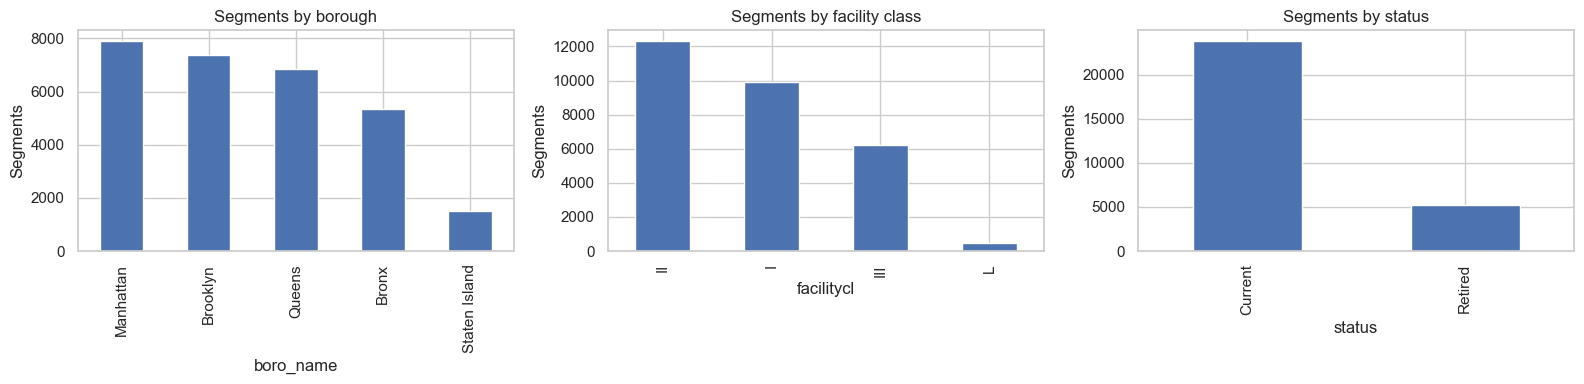
\includegraphics[width=\textwidth]{../media/segments_concentration.png}
  \caption{Breakdown of bike-lane segments by borough, facility class and status.}
  \label{fig:segments_concentration}
\end{figure}

The facility-class distribution distinguishes protected lanes from shared facilities and is used to style the network in the visualization.

The installation timeline illustrates the gradual expansion of the bike network over time, reflecting continued investment in cycling infrastructure. Figure~\ref{fig:installation_timeline} shows the number of installed segments over the years.

\begin{figure}[ptb]
  \centering
  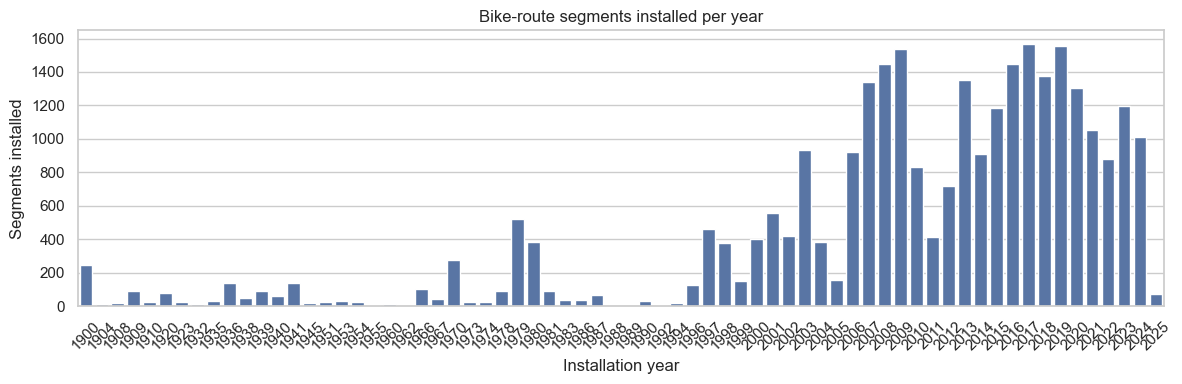
\includegraphics[width=\textwidth]{../media/installation_timeline.png}
  \caption{Bike-lane installation timeline.}
  \label{fig:installation_timeline}
\end{figure}

\subsection{Data Quality}

The dataset is generally clean but requires limited preprocessing.

Unused columns were removed to simplify the analysis without affecting the visualization.

Current and retired segments are treated separately so that obsolete infrastructure is not included in the active network layer.

Installation and retirement dates are occasionally missing, causing slight underestimation in historical summaries. When the installation date is unknown, NYC OpenData records the placeholder value \texttt{01/01/1900} instead of leaving it blank, so this sentinel year appears as the lower bound of the historical timeline.

Records with missing or invalid geometries cannot be displayed and are filtered before mapping. For the interactive visualization, only a sample of segments is rendered to improve responsiveness while preserving the overall spatial pattern.

\begin{comment}
    Possible future improvement: group facility classes into a smaller set of categories to simplify
    the legend and make the map easier to read.
    Possible future improvement: compare current and retired segments in separate layers to show how
    the network changed over time.
    Possible future improvement: enrich the network with contextual layers such as station density,
    trip hotspots, or transit corridors.
\end{comment}